\begin{wrapfigure}{r}{.5\textwidth} 
    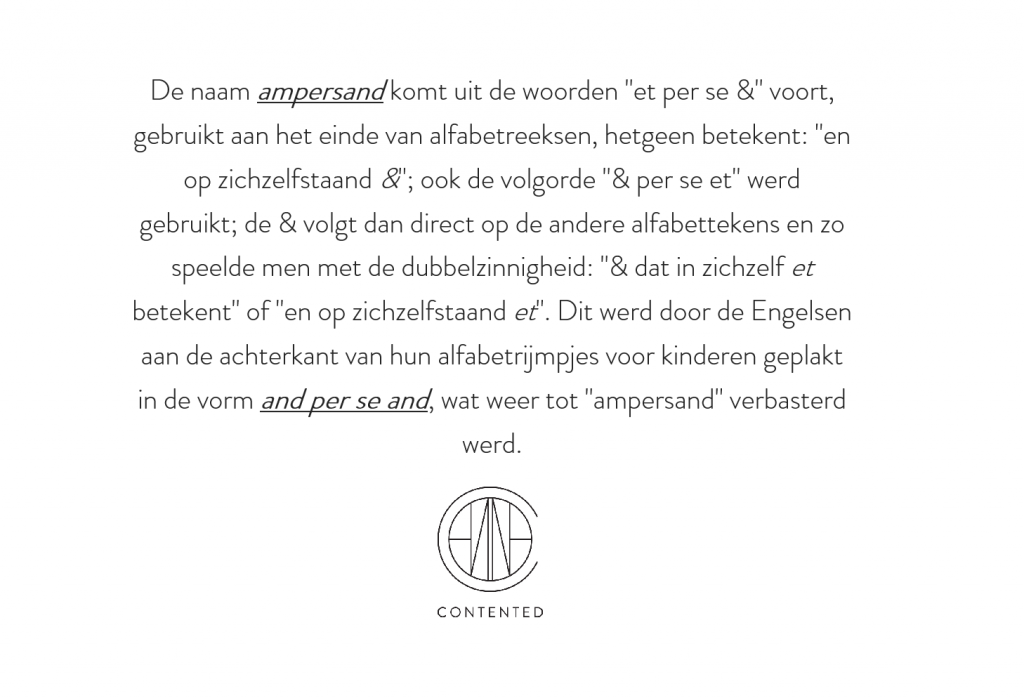
\includegraphics[scale=0.3]
        {Contented_Definitie_Ampersand_Wikipedia-1024x698.png}
    \caption{www.contented.nl/wat-weet-jij-van-het-en-teken-de-ampersand}
    \label{fig:Ampersand definition}
\end{wrapfigure}
The research focuses on the question of the usability of Ampersand, but where does Ampersand (\&) come from.
On the website of www.contend.nl~\footnote{\url{https://www.contented.nl/wat-weet-je-van-het-en-teken-de-ampersand}} we find an explanation for ampersand sign.
When applied to the Ampersand method, the similarity is that both emphasize the meaning "and self-contained".
The Ampersand method is a standalone method that is used.
On the website of 
Ampersand~\footnote{\url{https://ampersandtarski.gitbook.io/documentation/why-ampersand/business-rules-in-ampersand}} 
we find an interpretation of the statement "standalone (op zichzelfstaand)".
Ampersand endorses the \acrlong{brm}.
Elements are central here when focusing on primary requirements.
Do not let the process take center stage, but the facts.
In short, Ampersand its self-sufficiency follows the line of \&'s meaning.

During the graduation project, research was conducted into the suitability of Ampersand for designing registers for the government.
These registers are always based on legislation and regulations.
The research focuses on a specific law, namely the \acrshort{big}.

This law does not stand alone.
The associated laws and regulations are the following:
\begin{enumerate}
    \item Wet op de beroepen in de individuele gezondheidszorg;
    \item Algemene wet bestuursrecht;
    \item Besluit periodieke registratie Wet BIG;
    \item Registratiebesluit BIG;
    \item Tuchtrechtbesluit BIG;
    \item Besluit gezondheidszorgpsycholoog;
    \item Regeling periodieke registratie Wet BIG;
    \item Regeling tarieven registratie beroepsbeoefenaren Wet BIG;
    \item Algemene wet erkenning EU-beroepskwalificaties;
    \item Besluit buitenslands gediplomeerden volksgezondheid;
    \item Regeling erkenning EU-beroepskwalificaties beroepen in de individuele gezondheidszorg;
\end{enumerate} 

In principle, these laws and regulations are part of an investigation into the suitability of Ampersand.
However, the time that can be spent on the research does not allow to include all parts.
After all, the aim is not to provide a fully elaborated conceptual analysis.
By applying the principle of time-boxing, only a limited part of the legislation and regulations is analyzed and converted to Ampersand scripts.

The results of the study will be discussed in the following chapters.
The research that focuses on the research question "\acrlong{research question}".
By answering the derived questions, we provide a view on the usability of Ampersand.

The chosen approach of elaboration relates to the content analysis~\citep{kohlbacher_use_2006}.
Content analysis is a widely used research process.
It is a research method that converts qualitative data into quantitative figures.
This is done by reading and coding the qualitative data.
Qualitative data were obtained during the study in the form of notes and interviews.
Texts are assigned labels to show if there are important patterns in them.
Content analysis helps to see the amount of patterns in the data and to understand the connections between patterns.
The content analysis based on qualitative data as described by~\cite{kohlbacher_use_2006} is more often used in a case study.
The steps described by \cite{kohlbacher_use_2006} are also the steps followed within this \acrshort{ar}.
These concern according to \cite{kohlbacher_use_2006}:
\begin{enumerate}
    \item Collection evidence;
    \newline This was carried out by studying the legal texts and converting them in part to Ampersand.
    During this conversion, it was always recorded which observations had been made.
    \item Analyzing case study evidence;
    \newline This includes examining, categorizing and combining data.
    Here are several approaches~\citep{hsieh_three_2005}.
    Where the outcomes include relying on theoretical propositions, thinking about rival explanations of developing a case description.
    \item Reporting;
    \newline In the last step, the reporting of the findings takes place
\end{enumerate}
According to \cite{hsieh_three_2005} format, the "DIRECTED CONTENT ANALYSIS" is most applicable to this case.
The aim of direct content analysis is to validate a theory~\citep{hsieh_three_2005}.
The main goal of a focused approach is to help the researcher create developments.
Research would provide predictions about key variables and the relationships between them.
This will help find the encoding scheme.
Using a directed approach is more organized than using a conventional approach.
It starts with identifying key variables, after which operational definitions are determined per category.
Based on the research question, the data and the objectives of the researcher, the following strategy can be followed in labeling/coding.
The strategy starts with labeling using the predetermined codes.
In the process, information that could not be encoded is recognized and later analyzed to decide whether they represent a new category in the encoding scheme.
The existing theory is that Ampersand is very suitable for use in legislation and regulations.
And also for use within a government organization.
The impression is that the unfamiliarity in particular hinders the use and usefulness of Ampersand.
The collected data will show whether there is more here than the obscurity.
That is also the way in which the data will be classified and treated.
In addition, there have been discussions with stakeholders who fall within the analysis method of \cite{hsieh_three_2005} in the same way.
